\documentclass{article}


% if you need to pass options to natbib, use, e.g.:
%     \PassOptionsToPackage{numbers, compress}{natbib}
% before loading neurips_2022


% ready for submission
% \usepackage{neurips_2022}


% to compile a preprint version, e.g., for submission to arXiv, add add the
% [preprint] option:
    \usepackage[preprint]{neurips_2022}


% to compile a camera-ready version, add the [final] option, e.g.:
    % \usepackage[final]{neurips_2022}


% to avoid loading the natbib package, add option nonatbib:
%    \usepackage[nonatbib]{neurips_2022}


\usepackage[utf8]{inputenc} % allow utf-8 input
\usepackage[T1]{fontenc}    % use 8-bit T1 fonts
\usepackage{hyperref}       % hyperlinks
\usepackage{url}            % simple URL typesetting
\usepackage{booktabs}       % professional-quality tables
\usepackage{amsfonts}       % blackboard math symbols
\usepackage{nicefrac}       % compact symbols for 1/2, etc.
\usepackage{microtype}      % microtypography
\usepackage{xcolor}         % colors
\usepackage{graphicx}




\title{Cheating Detection in Zero-Sum Games for Mixed Multi-Agent Environments}

\author{%
  Aishik Pyne \\
  A0250592E\\
  \texttt{aipyne@comp.nus.edu.sg} \\
  % examples of more authors
  \And
   Harshavardhan Abichandani \\
  A0250610X\\
  \texttt{harsh@comp.nus.edu.sg} \\
  \And
   Niharika Shrivastava\\
  % \thanks{Use footnote for providing further information
  %   about author (webpage, alternative address)---\emph{not} for acknowledging
  %   funding agencies.} \\
  A0254355A\\
  \texttt{niharikacomp.nus.edu.sg} \\
}

\begin{document}
\maketitle

\begin{abstract}

Multi-agent reinforcement learning (MARL) is a prevalent learning paradigm for solving stochastic games. Specifically, imperfect information games model strategic interactions between multiple agents with only partial information which can be modelled as a POMDP \cite{pomdp:blog}. In most MARL studies, agents in a game are defined as teammates or enemies beforehand and these relationships among the agents are known to all. However, in real-world problems, the agent relationships are commonly unknown in advance. Therefore, training policies for such situations in the face of imperfect information and ambiguous identities is a significant problem that needs to be addressed. In this project, we aim to model the scenario for multi-agent partially-observable zero-sum games (e.g., poker, red-10) where M agents play collaboratively against (N-M) competitive agents. However, the (N-M) agents unknowingly assume a fully competitive setting. We also provide a discriminator that observes the entire game of all N agents and is able to detect cheating (a collaboration between M agents).

\end{abstract}

\section{Introduction}

Most AI systems nowadays are based on a single agent tackling a task, or in the case of adversarial models, multiple agents compete against each other to improve the overall behaviour of a system \cite{marl:blog}. However, many real-world scenarios require a mixed setting where multiple agents act either collaboratively or competitively with each other at different timesteps to get the best returns for themselves (e.g., driving a car to reach in the shortest time while avoiding creating traffic). 

In this aspect, multi-agent reinforcement learning (MARL) is a prevalent learning paradigm for solving stochastic games. Imperfect-information games model strategic interactions between multiple agents with only partial information (e.g., poker, blackjack, red-10). Typically in such games, one wishes to find an approximate equilibrium in which no player can improve by deviating from the equilibrium. Currently, the most successful algorithms for partially observable zero-sum games are Deep CFR \cite{dcfr:2018} and ReBel \cite{rebel:2020}. 

It is interesting to note that in most multi-agent works, whether an agent is acting collaboratively or competitively with other agents is known by everyone from the beginning which affects everyone's policies. However, in a real-life scenario, such an assumption may not always hold (e.g., a game of poker where 2 agents have teamed up against all other players with the intent of cheating). Therefore, we aim to model such a partially-observable mixed environment where individual agents attempt to maximize their reward assuming a fully competitive setting, but the teammates acting collaboratively are expected to win most games on average by maximizing their combined reward, at the expense of lower individual rewards. 

Such cheating scenarios are common in highly-dynamic, complex environments such as casinos. Therefore, we also train a cheating detector system that is able to observe the entire game state at all times along with the game-plays of every agent and is able to classify if there was any foul play during the game. 

\section{Problem Definition}

In this project, we aim to achieve the following 3 goals:

\begin{enumerate}
    \item Implement a multi-agent zero-sum game playing AI where the policy for each agent is learned in a fully-competitive setting using common off-the-shelf RL methods, such as CFR, SAC, ReBeL.

    \item Implement a multi-agent zero-sum game playing AI where 2 agents play collaboratively against N competitive players in order to beat them in most games. Just as in a real-life case, each player's game space is still partially observable but the expected team reward is maximized.

    \item Model a discriminator that learns to distinguish between these two styles of play (fair vs foul) by observing the actions taken by the players and the overall game state. 
\end{enumerate}

All the environments can be defined as a Partially Observable Markov Decision Process (POMDP) which is described as a tuple $\langle S, A, T, R, O, \Omega \rangle$ where:
\begin{itemize}
    \item S - finite set of states of the environment, (game space)
    
    \item A - finite set of actions (raise, fold, call, check).
    
    \item $T: S$ x $A \rightarrow \Delta(S)$ - state-transition function, giving a distribution over states of the environment, given a starting state and an action performed by the agent.
    
    \item R -  the reward function, giving a real-values expected immediate reward, given a starting state and an action performed by the agent. (money/chips after every move)
    
    \item $\Omega$ - finite set of observations the agent can experience
    
    \item $O: S$ x $ A \rightarrow \Delta(\Omega)$ -  the observation function, giving a distribution over possible observations, given a starting state and an action performed by the agent.
\end{itemize}

\section{Literature Review}

There are many approaches developed for finding nash equilibrium in games with imperfect information \cite{rebel:2020, dcfr:2018, nsfp:2016, deepstack}. We will be focusing on the two most popular approaches, Neural Fictitious Self Play and Deep Counterfactual Regret Minimization.

Neural Fictitious Self Play (NFSP) \cite{nsfp:2016} is one of the algorithms used to train agents for imperfect information games (eg. poker) which combines fictitious self play with neural networks. During training, the agent plays against itself. The algorithm consists of two memory buffers, first contains the experience collected from playing other agents. This memory is used to predict the value of the actions taken by the agent. Second, contains the experience of agent's own behaviour which is used to keep track of its own average behavior.

Deep Counterfactual Regret Minimization (Deep CFR) \cite{dcfr:2018}, it combines CFR with neural networks. It builds on CFR which traverses the search space and accumulates the regrets at each stage. Strategy is chosen based on algorithms which work on the principle of regret minimization. CFR cannot be used to for games with large state space, to solve this Deep CFR uses neural networks to approximate the rest of the state space. In Deep CFR at every iteration the game tree is partially traversed $K$ times and the paths are sampled using MCCFR. After the traversals, a neural network is used to predict the value of exploring that node. This can be thought of as instantaneous regrets in the CFR algorithm. 

The above methods consider only one to one competitive play, for problems with mixed environment having $N \geq 3$ players the most popular algorithm is MADDPG \cite{maddpg}. MADDPG works by having a centralized critic that is trained using global observation and the private observation of the agents, but at test time the agents only act on the local information.

\section{Methodology}

For this project, we set up a game table of 3 agents according to the below-mentioned settings. All the agents have the objective to maximize their individual or team reward according to their role in the setting (competitive or collaborative respectively). The reward is defined as the money it earns from playing an entire game. If the model is modelled successfully, it is expected to have super-human performance against human/sub-par players. However, when the agents play against themselves (self-play), it should converge to a nash-equilibrium. All the settings below can be defined as a Partially Observable Markov Decision Process (POMDP) which is described as a tuple $\langle S, A, T, R, O, \Omega \rangle$.

\begin{figure}[h]
    \centering
    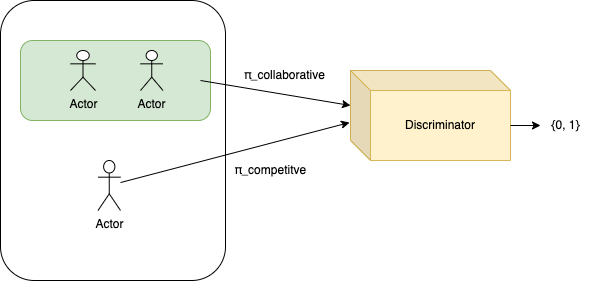
\includegraphics[width=10cm]{./images/framework.png}
    \caption{Cheating Detection for Mixed Multi-Agent Environments}
    \label{fig:cheating}
\end{figure}

It is important to note that we can increase the number of agents and implement this framework for any zero-sum partially observable game and expect successful outcomes. Currently, we are using poker and open-source implementations to evaluate our results.

\subsection{Fully Competitive Environment Setting}

All 3 agents play against each other with the objective to maximize their individual rewards. We train each agent using Deep CFR \cite{dcfr:2018} or NFSP \cite{nsfp:2016} using the OpenSpiel \cite{openspiel:2019} RLCard library \cite{rlcard}. 

\subsection{Mixed Environment Setting}

Once the fully competitive AI policy has reached optimality, it can be treated as a baseline. Two agents are teammates and play collaboratively to maximize their total reward, while the third agent plays competitively against them to maximize its individual reward, without knowing that they are teammates. This means one teammate can learn to sacrifice its reward as long as the total team reward is maximized. We model this by additionally providing the teammates access to each other's hands (cards) during training as input. However, during test time the teammates have access to only their hand cards. 

We are currently exploring methods to use open-sourced implementations of Deep CFR, or MADDPG \cite{maddpg} using either OpenSpiel or the RLCard library. 

\subsection{Discriminator}

For training, the discriminator observes the difference in trajectories of the collaborative and the competitive agents and predicts if any foul play occurred during the game.

The trajectories of each agent have multiple features such as legal actions, observations, actions taken, etc. These are fed into a GRU to get a representative embedding for each agent for a single game. We then create a dataset of multiple such trajectories by playing N games. Then the discriminator is trained on this dataset using any off-the-shelf supervised learning algorithm for binary classification such as a Naive Bayes Classifier or MLP to predict if a policy was collaborative or competitive.

This discriminator would have practical use cases of being a cheating detector in games but also a generic way to observe divergence in policies.

\section{Evaluation Metric}

We are utilizing three metrics to evaluate our trained agents which are Win Rate, Best Response and Head to Head. 

The following metrics are used to evaluate our trained agents.

\begin{enumerate}
    \item Win Rate: The single agent will play against a randomly initialized policy and on expectation the trained policy should accumulate higher rewards.

    \item Best Response: In this metric, multiple games will be simulated and at each level of the sub tree, utility of the trained agent's actions are compared against the best response action. For games like poker where the state space is high and sub trees cannot be generated, we will be using an approximation of the best response. The approximate value is generated by finding the lower bound \cite{lowerbound} or by training a DDQN \cite{br_ddqn}. 

    \begin{center}
        $$S = \mathcal{U}(\pi_{\text{competitive}}(a)) - \mathcal{U}(\pi_{\text{BR}}(a))$$
    \end{center}

    \item Head to Head: The trained agent will play aginst a pretrained agent. The pretrained agent's policy will be trained using current open source implementations. In this mode it is possible for the agents to achieve nash equilibrium.
\end{enumerate} 


To evaluate the performance of the discriminator we are using accuracy on the unseen dataset as our metric. The dataset will contain trajectories from the competitive agent policy $\pi_{\text{competitive}}$ and the collaborative agents policies $\pi_{\text{collaborative}}$.

\section{Expected Outcome}

% Mention what outcomes you are expecting using the above evaluation metrics

The purpose of this project is to build a framework to detect which agents in the environment are collaborating. 

\subsection{Competitive Environment Setting} 
In this setting we are expecting the single agent to outperform a randomly initialized policy on average. Moreover, we are expecting agents trained using Deep CFR to outperform agents trained using CFR or NFSP. This outcome will be consistent with the existing literature.

\subsection{Mixed Environment Setting}
We are working on the simplest setting where there are three agents in total. Two agents will be collaborating against the third agent. In this, a successful implementation will result in collaborative agents accumulating more rewards in expectation than the third agent. For games like poker this means that the two agents colluding will have more chips. This is consistent with real life because the two agents are making decisions using additional information.

\subsection{Discriminator}
Based on our current implementation of the discriminator we are expecting it to accurately discriminate between actions taken by collaborative agents and competitive agents.

\newpage 

\section{Timeline}

\begin{enumerate}
    \item \textbf{Week 11}: Train and evaluate fully-competitive setting for multi-agents.

    \item \textbf{Week 12}: Train and evaluate mixed setting for multi-agents. 

    \item \textbf{Week 13}: Train a discriminator to detect the divergence between collaborative and competitive policies.

    \item \textbf{Week 14}: Report writing and presentation.
\end{enumerate}

\newpage

\bibliographystyle{plain}
\bibliography{refs}

% \section*{References}

% {
% \small
% [1] Brown, N., Bakhtin, A., Lerer, A., \& Gong, Q. (2020). Combining deep reinforcement learn- ing and search for imperfect-information games. CoRR, abs/2007.13544.
% }

\end{document}
